\documentclass[a4paper,12pt,portuguese]{report}
\usepackage[utf8]{inputenc}
\usepackage[portuguese]{babel}
\usepackage{ragged2e}
\usepackage{fancyvrb}
\usepackage{graphicx}

\title{Projeto do grupo 40 \\ Programação Orientada aos Objectos}
\author{Martins, José(a78821)\
        \and
        Costa, Mariana(a78824)\
        \and
        Quaresma, Miguel(a77049)
        }
\date{\today}

\begin{document}
 
\begin{titlepage}
\maketitle
\end{titlepage}
 
\tableofcontents
 
\chapter{Introdução}
\textbf{UmER} é uma aplicação para transporte de passageiros e que permite que um utilizador realize viagens em táxis da UmER. Esta(aplicação) providencia mecanismos de criação de contas (de passageiros e motoristas), automóveis, realização de viagens e consulta das mesmas, alteração do estado dos motoristas(disponíveis ou indisponíveis). A aplicação permite ainda a permanência de dados aquando o fecho da mesma e a recuperação de um esado previamente guardado.

\chapter{Desenvolvimento}

\section{Arquitetura de Classes}

\begin{figure}[ht!]
    \centering
        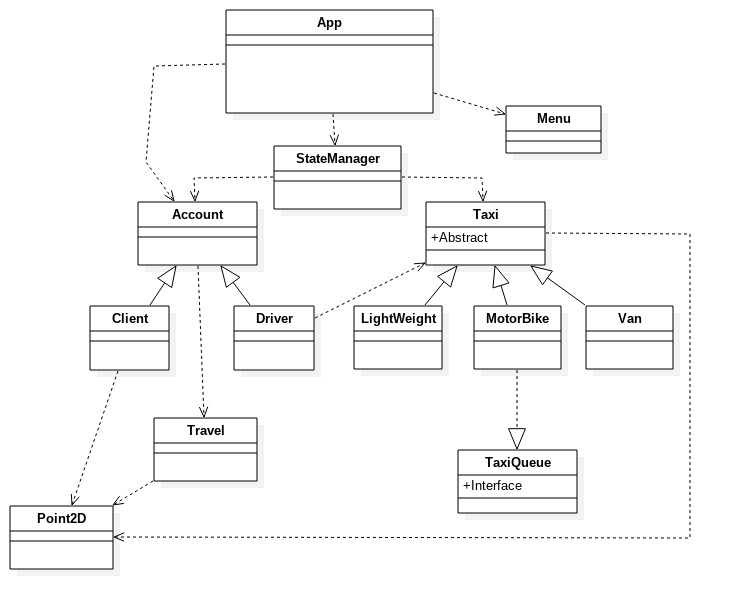
\includegraphics[width=120mm]{graph.jpg}
    \caption{Principais Classes}
\end{figure}

Em termos de classes, como podemos visualizar na imagem acima, temos uma classe principal(App) que "controla" tudo, dependendo por composição das classes StateManager, Account e Menu.

\section{Aplicação e suas funcionalidades}

\section{Como seria possível adicionar novos tipos de viaturas e motoristas na aplicação?}

Para adicionar novas viaturas basta criar a classe da mesma e torná-la subclasse da classe abstrata Taxi. Contudo quanto a adicionar novos tipos de motorista n seria tão fácil, pois seria necessário, tornar a classe motorista como abstrata e a partir daí pôr os novos tipos de motoristas como subclasse dessa.

\chapter{Conclusão}
Devio a alguns contratempos acabamos por nao implementar as companhias/empresas de taxis nem suas funções subjacentes(p.e. indicar o total faturado por uma viatura, ou empresa de táxis, num determinado período), porém com a atual estrutura do projeto é viável de se concretizar.

\end{document}
